\documentclass{beamer}
\usepackage[utf8]{inputenc}
\usepackage[T1]{fontenc}
\usepackage[catalan]{babel}
\usepackage{amsmath}
\usepackage{amssymb}
\usepackage{amsthm}

\newtheorem{teorema}{Teorema}
\newtheorem{corollari}{Corol\textperiodcentered lari}
\newtheorem{lema}{Lema}
\newtheorem{definicio}{Definici\'{o}}
\newtheorem{notacio}{Notaci\'{o}}
\newtheorem{proposicio}{Proposici\'{o}}
\newtheorem{observacio}{Observaci\'{o}}
\theoremstyle{definition}
\newtheorem{exemple}{Exemple}

\mode<presentation>
{
\usetheme{Boadilla}
\usecolortheme{seahorse}
}

\title{Ones viatgeres}
\author{Alejandro Plaza Gall\'{a}n}
\date{8 de juny de 2021}

\begin{document}

\begin{frame}
\titlepage
\end{frame}

\begin{frame}{Introducci\'{o}}
Partim de l'\textbf{equaci\'{o} d'ones} unidimensional cl\`{a}ssica.
\[\frac{\partial^2u}{\partial t^2}-c^2\frac{\partial^2u}{\partial x^2}=0\]
\pause
Aquesta equaci\'{o} en derivades partials descriu la posici\'{o} dels punts d'una corda vibrant, on $u$ \'{e}s el despla\c{c}ament dins l'oscil\textperiodcentered laci\'{o}, $x$ \'{e}s la posici\'{o} dins la corda i $t$ \'{e}s el temps.
\pause

Algunes solucions particulars d'aquesta equaci\'{o} s\'{o}n les funcions de la forma
\[\varphi(x-ct)\hspace{3mm}\text{o}\hspace{3mm}\varphi(x+ct),\]
on $\varphi$ \'{e}s una funci\'{o} $C^2$ qualsevol.
\pause

Les funcions d'aquesta forma es diuen \textbf{ones viatgeres}.
\end{frame}

\begin{frame}{Exist\`{e}ncia d'ones viatgeres}
L'objectiu \'{e}s trobar ones viatgeres com a solucions de diferents equacions diferencials.
\pause
\[u_t=u_{xx}+f(u),\]
\pause
on
\begin{enumerate}
\item $f(0)=0$,
\pause
\item $f(1)=0$,
\pause
\item $f(u)>0$ per $0<u<1$,
\pause
\item $f''(u)<0$.
\end{enumerate}
\pause
L'equaci\'{o} de Fisher-Kolmogorov \'{e}s el cas particular que $f(u)=u(1-u)$.
\end{frame}

\begin{frame}{Exist\`{e}ncia d'ones viatgeres}
Busquem llavors solucions de la forma $u=U(x-ct)$. Volem una ona viatgera de tipus front, que comenci l'$1$, decreixi cap a l'$0$ i es mogui cap a la dreta.
\begin{figure}[ht!]
\begin{center}
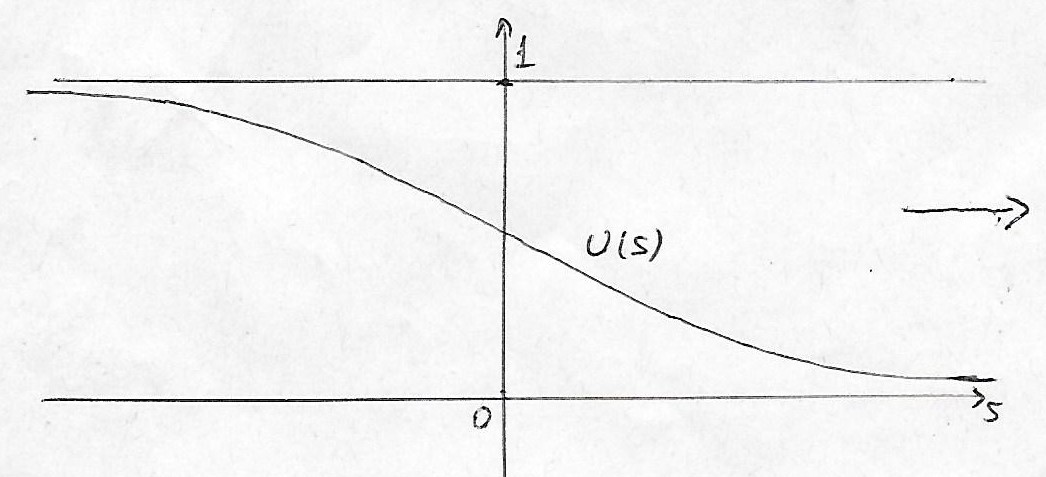
\includegraphics[width=8cm]{Front.jpg}
\end{center}
\end{figure}
\end{frame}

\begin{frame}{Exist\`{e}ncia d'ones viatgeres}
\[u_t=u_{xx}+f(u)\]
\'{E}s clar que $u=0$ i $u=1$ s\'{o}n solucions trivials. Busquem llavors solucions no trivials, pel qual substitu\"{i}m $u$ per $U(x-ct)$ en l'equaci\'{o} de Fisher-Kolmogorov. \pause Calculant
\[\frac{\partial u}{\partial t}=-cU'(x-c)\hspace{3mm}\text{i}\hspace{3mm}\frac{\partial^2u}{\partial x^2}=U''(x-c),\]
\pause
obtenim l'equaci\'{o}
\[U''+cU'+f(U)=0,\]
la qual \'{e}s una equaci\'{o} diferencial de segon ordre no lineal. \pause La podem transformar en l'EDO de primer ordre seg\"{u}ent:
\[\left\{\begin{array}{ll}U'=V,\\V'=-cV-f(U).\end{array}\right.\]
\end{frame}

\begin{frame}{Exist\`{e}ncia d'ones viatgeres}
\[\left\{\begin{array}{ll}U'=V,\\V'=-cV-f(U).\end{array}\right.\]
Els punts cr\'{i}tic d'aquest sistema els obtenim resolent
\[\left\{\begin{array}{l}U'=0,\\V'=0,\end{array}\right.\]
\pause
i s\'{o}n els punts
\begin{itemize}
\item $P_1=(0,0)$,
\item $P_2=(1,0)$.
\end{itemize}
\pause
Estudiem el tipus de punt cr\'{i}tic mitjan\c{c}ant el teorema de Hartman calculant la matriu jacobiana del camp $X$.
\pause
\[DX(U,V)=\left(\begin{matrix}0&1\\-f'(U)&-c\end{matrix}\right)\]
\end{frame}

\begin{frame}{Exist\`{e}ncia d'ones viatgeres}
\[DX(1,0)=\left(\begin{matrix}0&1\\-f'(1)&-c\end{matrix}\right)\]
\pause
De les condicions de $f$ es dedueix que ha de ser $f'(1)<0$, implicant que $\det(DX(1,0))=f'(1)<0$. Per tant ha de tenir un valor propi positiu i una altre negatiu. Pel teorema de Hartman, el $(1,0)$ \'{e}s una sella.
\pause
\[DX(0,0)=\left(\begin{matrix}0&1\\-f'(0)&-c\end{matrix}\right)\]
\pause
El polinomi caracter\'{i}stic \'{e}s
\[\left|\begin{matrix}\lambda&-1\\f'(0)&\lambda+c\end{matrix}\right|=\lambda^2+c\lambda+f'(0).\]
\pause
Les arrels s\'{o}n
\[\lambda=\frac{-c\pm\sqrt{c^2-4f'(0)}}{2}.\]
\end{frame}

\begin{frame}{Exist\`{e}ncia d'ones viatgeres}
Si el discriminant
\[c^2-4f'(0)\]
\'{e}s negatiu, \'{e}s a dir, si $|c|<2\sqrt{f'(0)}$, llavors els valors propis seran complexos i el $(0,0)$ ser\`{a} un focus.
\pause

Si, en canvi, el discriminant \'{e}s no negatiu, o equivalentment, $|c|\geq2\sqrt{f'(0)}$, aleshores els valors propis seran reals.
\pause

Si $c>0$, seran  valors propis negatius i tindrem un node atractor a $P_1$. Si $c<0$, seran negatius i $P_1$ ser\`{a} un node repulsor.
\pause

Per la hip\`{o}tesi de ser $U$ una ona viatgera de tipus front, ha de ser $c>2\sqrt{f'(0)}$. Per tant el $(0,0)$ \'{e}s un node atractor.
\end{frame}

\begin{frame}{Exist\`{e}ncia d'ones viatgeres}
Hi haur\`{a} una ona viatgera de tipus front si i nom\'{e}s si hi ha una \`{o}rbita heterocl\'{i}nica que vagi de la sella $(1,0)$ al node atractor $(0,0)$.
\pause

Per aconseguir-ho, tancarem la separatriu inestable de la sella dins d'una regi\'{o} positivament invariant.
\pause

Fem el canvi de variable $x=1-U,y=V$ i escrivim $g(x)=-f(1-x)$. L'EDO ens queda:
\[\left\{\begin{array}{l}x'=-y,\\y'=-cy+g(x).\end{array}\right.\]
\end{frame}

\begin{frame}{Exist\`{e}ncia d'ones viatgeres}
Prenem la fam\'{i}lia de corbes
\[G_{\lambda}(x,y)=y-\lambda g(x)=0.\]
\pause
\begin{figure}[ht!]
\begin{center}
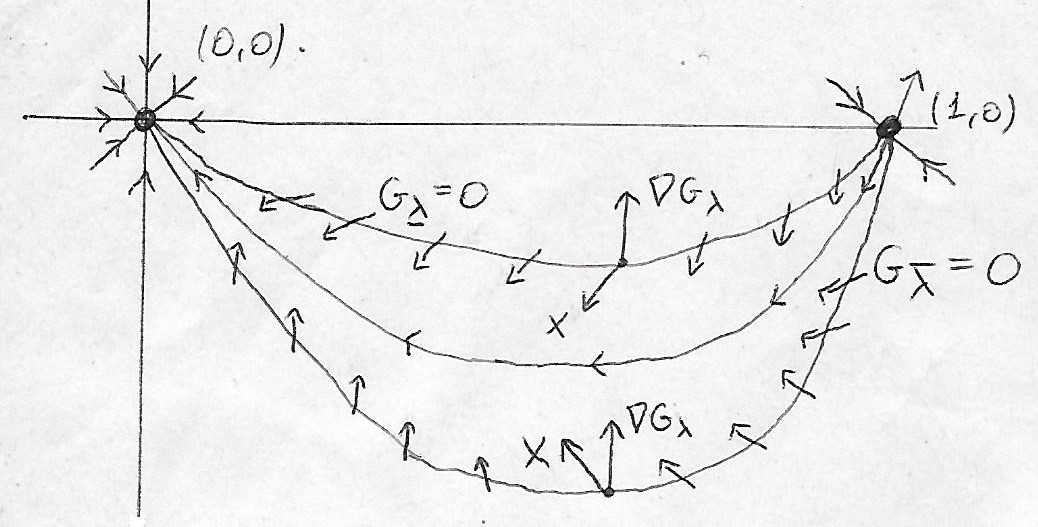
\includegraphics[width=10cm]{Lluna.jpg}
\end{center}
\end{figure}
\end{frame}

\begin{frame}{Exist\`{e}ncia d'ones viatgeres}
\[\langle\nabla G_{\lambda}(x,\lambda g(x)),X(x,\lambda g(x))\rangle=g(x)(1-c\lambda+g'(x)\lambda^2)=g(x)N_{\lambda}(x)\]
\pause
Com que $g(x)\leq0$, el signe de $\langle\nabla G_{\lambda},X\rangle$ ser\`{a} el contrari del de $N_{\lambda}(x)$.
\pause

A m\'{e}s $N_{\lambda}'(x)=g''(x)\lambda^2>0$, pel qual $N_{\lambda}(x)$ \'{e}s creixent. Aix\'{i} doncs, si $N_{\lambda}(0)=0$, tindrem $N_{\lambda}(x)\geq0$ i si $N_{\lambda}(1)=0$, tindrem $N_{\lambda}(x)\leq0$.
\pause

Siguin $\underline\lambda$ i $\overline\lambda$ tals que
\[N_{\underline\lambda}(0)=1-c\underline\lambda+g'(0)\underline\lambda^2=0,\]
\[N_{\overline\lambda}(1)=1-c\overline\lambda+g'(1)\overline\lambda^2=0.\]
\end{frame}

\begin{frame}{Exist\`{e}ncia d'ones viatgeres}
\begin{figure}[ht!]
\begin{center}
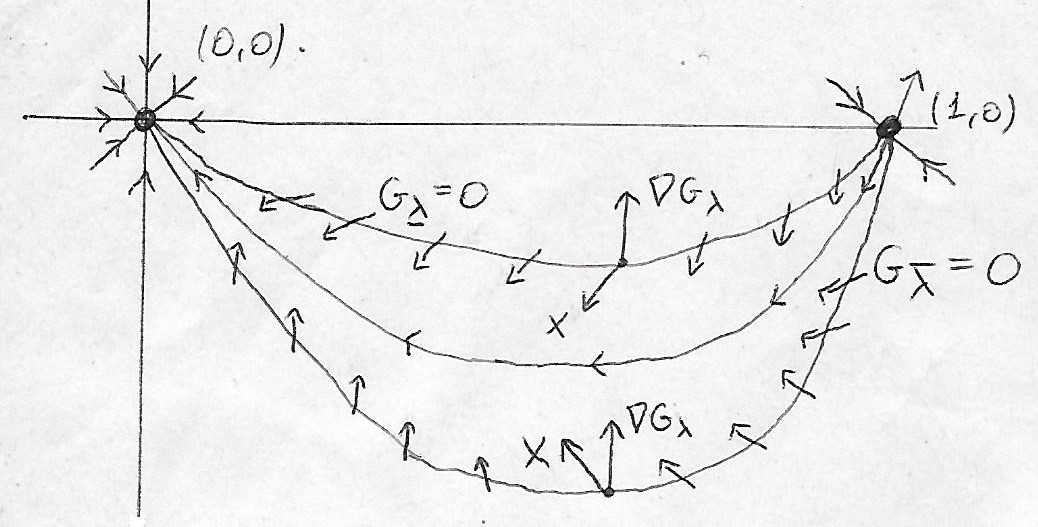
\includegraphics[width=9cm]{Lluna.jpg}
\end{center}
\end{figure}
Amb aix\`{o} llavors entre les corbes $G_{\underline\lambda}(x,y)=0$ i $G_{\overline\lambda}(x,y)=0$ es troba una regi\'{o} positivament invariant. En conclusi\'{o}, la separatriu inestable de la sella no podr\`{a} sortir de la regi\'{o}. Per tant, ha d'estar tota ella continguda a la regi\'{o} invariant. \pause Ara, pel teorema de Poincar\'{e}-Bendixson, el seu $\omega$-l\'{i}mit no pot ser buit i per tant ha de contenir un punt cr\'{i}tic, que ser\`{a} el $(0,0)$.
\end{frame}

\begin{frame}{Pertorbacions}
Prenem $f(u)=u(1-u)$ i la pertorbem canviant-la per $u(1-u)(u-a)$ amb $0<a<1$.
\pause
\[\left\{\begin{array}{l}U'=V,\\V'=-cV-U(1-U)(U-a).\end{array}\right.\]
\pause
Hi ha tres punts cr\'{i}tics: $(0,0)$, que ser\`{a} una sella, el $(a,0)$, que ser\`{a} un centre, node o focus, i el $(1,0)$, que ser\`{a} una altra sella. Per tant trobarem una connexi\'{o} entre les selles.
\begin{figure}[ht!]
\begin{center}
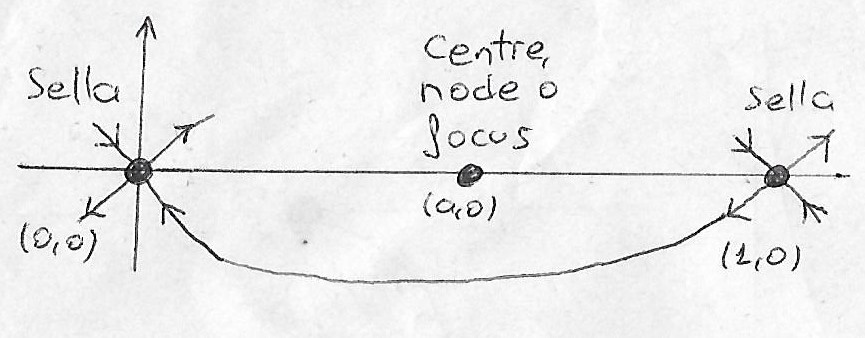
\includegraphics[width=10cm]{Critics.jpg}
\end{center}
\end{figure}
\end{frame}

\begin{frame}{Pertorbacions}
Veurem que hi ha un \'{u}nic $c>0$ pel qual existeix una connexi\'{o} heterocl\'{i}nica i, conseg\"{u}entment, una ona viatgera de tipus front.
\pause
\begin{definicio}
Una fam\'{i}lia de camps $X((x,y),c)=(P((x,y),c),Q((x,y),c))$ es diu \textbf{rotat\`{o}ria} quan
\[PQ_c-P_cQ\]
no canvia de signe i no \'{e}s id\`{e}nticament zero.
\end{definicio}
\pause
La motivaci\'{o} \'{e}s que $PQ_c-P_cQ$ t\'{e} el signe de la variaci\'{o} de l'angle del camp, com veiem a la seg\"{u}ent f\'{o}rmula.
\[\theta(c)=\arctan\frac{Q}{P};\hspace{7mm}\theta'(c)=\frac{PQ_c-P_cQ}{P^2+Q^2}.\]
\end{frame}

\begin{frame}{Pertorbacions}
Si hi ha una connexi\'{o} heterocl\'{i}nica entre dues selles per un cert $c$, en pertorbar-lo una mica, s'ha de trencar la connexi\'{o} ja que les dues noves branques no poden creuar la antiga connexi\'{o}.
\begin{figure}[ht!]
\begin{center}
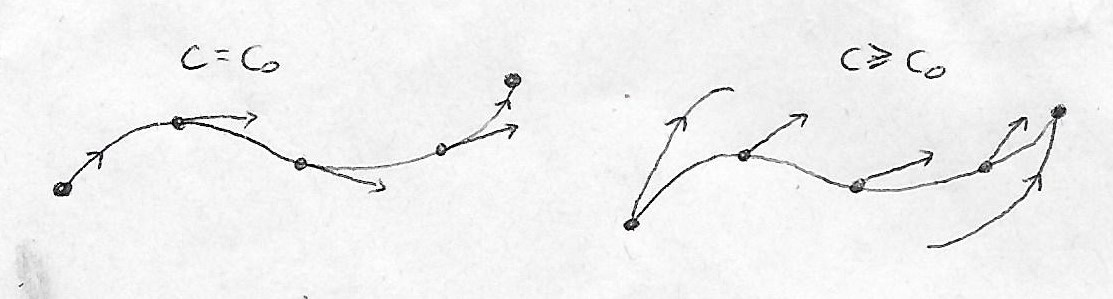
\includegraphics[width=10cm]{Trencament.jpg}
\end{center}
\end{figure}
\pause
\[\left\{\begin{array}{l}U'=P((U,V),c)=V,\\V'=Q((U,V),c)=-cV-U(1-U)(U-a),\end{array}\right.\]
\[PQ_c-P_cQ=-V^2<0.\]
\pause
Per tant \'{e}s una fam\'{i}lia rotat\`{o}ria i existir\`{a} com a molt un \'{u}nic $c$ pel qual hi hagi una connexi\'{o} heterocl\'{i}nica.
\end{frame}

\begin{frame}{Pertorbacions}
\begin{figure}[ht!]
\begin{center}
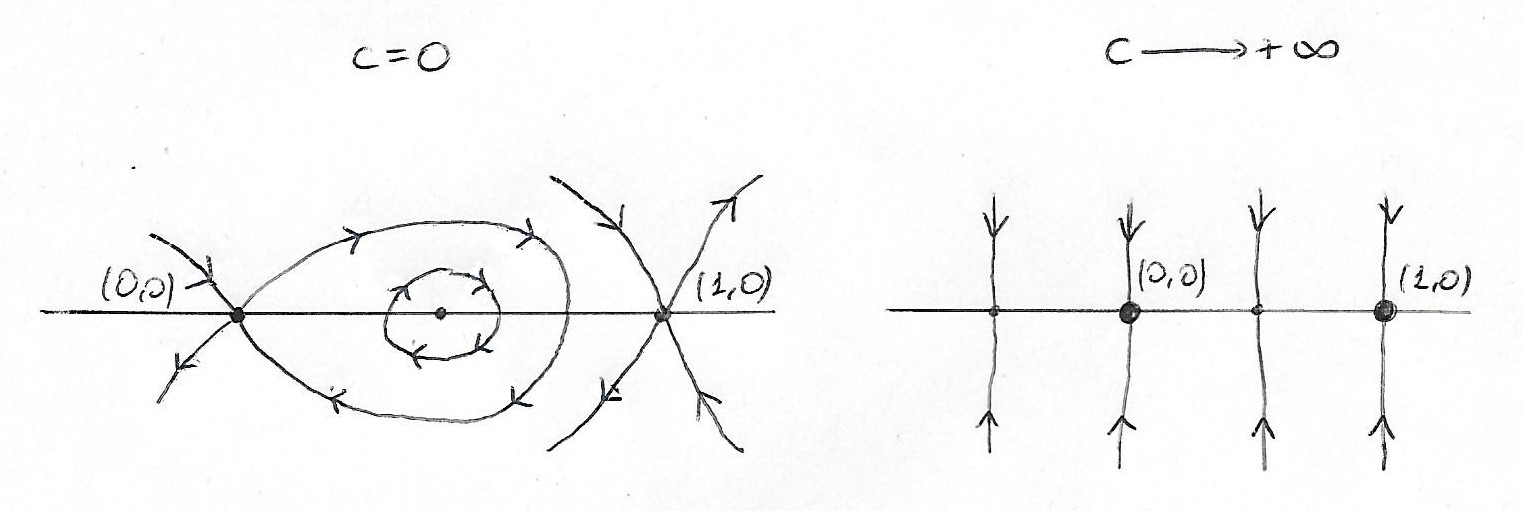
\includegraphics[width=9cm]{Limit.jpg}
\pause
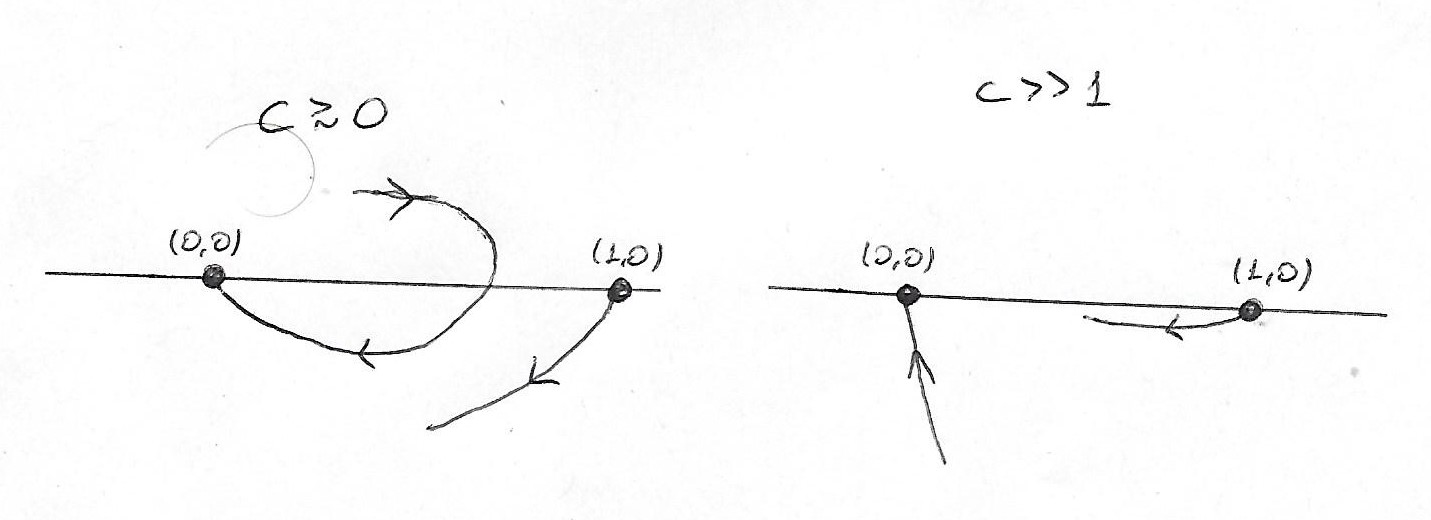
\includegraphics[width=9cm]{Proper.jpg}
\end{center}
\end{figure}
\pause
Com que tenim una fam\'{i}lia rotat\`{o}ria, en algun $c$ es trobaran les dues separatrius de les dues selles i formaran una connexi\'{o}.
\end{frame}

\begin{frame}{Solucions algebraiques}
Tornant a l'equaci\'{o} de Fisher-Kolmogorov,
\[U''+cU'+U(1-U)=0,\]
si $c=\frac{5}{\sqrt{6}}$, per $k>0$, Ablowitz and Zeppetella van provar que existeix la soluci\'{o}
\[U(s)=\frac{1}{\left(1+ke^{\frac{s}{\sqrt{6}}}\right)^2},\]
que d\'{o}na lloc a una ona viatgera de velocitat $c=\frac{5}{\sqrt{6}}$.
\pause

S'han trobat tamb\'{e} d'altres ones viatgeres per altres equacions diferencials i totes elles tenen la forma
\[U(s)=\frac{q_1(e^{\lambda s})}{q_2(e^{\lambda s})},\]
on $\lambda\in\mathbb{R}$ i $q_1,q_2$ s\'{o}n polinomis reals.
\end{frame}

\begin{frame}{Solucions algebraiques}
\begin{definicio}
Diem que $U(s)$ \'{e}s una \textbf{soluci\'{o} algebraica} quan existeix un polinomi $p\in\mathbb{R}[x,y]$ no nul tal que $p(U(s),U'(s))=0$.
\end{definicio}
\pause
\begin{lemma}
Si $U(s)$ \'{e}s una funci\'{o} racional amb variable exponencial:
\[U(s)=\frac{q_1(e^{\lambda s})}{q_2(e^{\lambda s})},\]
aleshores existeix un polinomi $p\in\mathbb{R}[x,y]$ tal que $p(U(s),U'(s))=0$.
\end{lemma}
\end{frame}
\end{document}
